% !TEX root = ../main.tex
% File: chapters_part1/chap1_intro.tex
% Nội dung cho Chương 1 của Phần 1


\section{Định nghĩa và Phạm vi}
\label{sec:dinh_nghia_pham_vi}

Trước khi đi sâu vào các thuật toán phức tạp hay những mô hình khổng lồ, việc đầu tiên và quan trọng nhất là phải trả lời được câu hỏi: "Chính xác thì chúng ta đang nghiên cứu về cái gì?". Mục này sẽ vạch ra ranh giới, định nghĩa và phạm vi của ngành Xử lý Ngôn ngữ Tự nhiên.

\subsection{Xử lý Ngôn ngữ Tự nhiên (NLP) là gì?}
\label{ssec:nlp_la_gi}

Một cách tổng quát nhất, Xử lý Ngôn ngữ Tự nhiên là một lĩnh vực liên ngành của Trí tuệ Nhân tạo (AI), Khoa học Máy tính và Ngôn ngữ học, tập trung vào việc trao cho máy tính khả năng \textbf{hiểu, diễn giải, xử lý và tạo ra ngôn ngữ của con người} (dưới dạng văn bản hoặc giọng nói) theo một cách có giá trị và hữu ích.

Mục tiêu cuối cùng của NLP không chỉ dừng lại ở việc xử lý các chuỗi ký tự, mà là thu hẹp khoảng cách giao tiếp giữa con người và máy tính. Chúng ta muốn máy tính không chỉ "đọc" được văn bản, mà còn "hiểu" được ý nghĩa, ngữ cảnh, cảm xúc, và thậm chí cả những ẩn ý đằng sau con chữ.

\begin{definition}{Xử lý Ngôn ngữ Tự nhiên (NLP)}{def:nlp}
    NLP là một lĩnh vực của Trí tuệ Nhân tạo nhằm mục đích xây dựng các hệ thống tính toán có khả năng xử lý và hiểu được ngôn ngữ tự nhiên của con người để thực hiện các tác vụ hữu ích.
\end{definition}

Lĩnh vực NLP bao gồm hai khía cạnh chính, thường hoạt động song hành với nhau:

\begin{itemize}
    \item \textbf{Hiểu Ngôn ngữ Tự nhiên (Natural Language Understanding - NLU):} Đây là khía cạnh tập trung vào việc "đọc hiểu" của máy tính. NLU bao gồm các bài toán yêu cầu máy tính phân tích và rút ra ý nghĩa từ một đoạn văn bản. Các nhiệm vụ như phân tích cú pháp, nhận dạng thực thể, hay phân tích cảm xúc đều thuộc về NLU.
    
    \item \textbf{Sinh Ngôn ngữ Tự nhiên (Natural Language Generation - NLG):} Đây là khía cạnh tập trung vào việc "viết" hoặc "nói" của máy tính. NLG bao gồm các bài toán yêu cầu máy tính tự động tạo ra một đoạn văn bản mạch lạc, tự nhiên và phù hợp với ngữ cảnh. Các nhiệm vụ như dịch máy, tóm tắt văn bản, hay xây dựng các chatbot trả lời tự động đều là ví dụ điển hình của NLG.
\end{itemize}

Thử thách lớn nhất của NLP nằm ở chính bản chất phức tạp và mơ hồ của ngôn ngữ tự nhiên. Ngôn ngữ của con người không tuân theo các quy tắc logic chặt chẽ như ngôn ngữ lập trình. Nó đầy rẫy sự đa nghĩa (một từ có nhiều nghĩa), phụ thuộc vào ngữ cảnh, chứa đựng tiếng lóng, sai sót chính tả, và liên tục biến đổi. Việc mô hình hóa và xử lý được những đặc tính này chính là trọng tâm của ngành.

\begin{example}{Một số ứng dụng thực tế của NLP}{ex:ung_dung_nlp}
    Để hình dung rõ hơn, hãy xem xét các ứng dụng của NLP mà chúng ta tương tác hàng ngày:
    \begin{itemize}
        \item \textbf{Máy tìm kiếm (Search Engines):} Google, Bing sử dụng NLP để hiểu câu truy vấn của bạn (dù bạn gõ sai chính tả hay dùng từ ngữ thông tục) và trả về các kết quả liên quan nhất.
        \item \textbf{Trợ lý ảo (Virtual Assistants):} Siri, Google Assistant, và Alexa dùng NLP để hiểu mệnh lệnh bằng giọng nói và sinh ra câu trả lời phù hợp.
        \item \textbf{Dịch tự động (Machine Translation):} Google Translate có thể dịch tức thời giữa hàng trăm ngôn ngữ.
        \item \textbf{Phân tích cảm xúc (Sentiment Analysis):} Các công ty phân tích các bình luận trên mạng xã hội để biết khách hàng đang nghĩ gì về sản phẩm của họ.
        \item \textbf{Tự động sửa lỗi và gợi ý văn bản (Autocorrect \& Predictive Text):} Tính năng bạn dùng hàng ngày trên điện thoại và trình soạn thảo văn bản.
        \item \textbf{Chatbots hỗ trợ khách hàng:} Tự động trả lời các câu hỏi thường gặp, giúp giảm tải cho nhân viên hỗ trợ.
    \end{itemize}
\end{example}

\subsection{Mối quan hệ với Trí tuệ Nhân tạo, Học máy và Ngôn ngữ học}
\label{ssec:moi_quan_he}

NLP không tồn tại một cách độc lập. Nó là một giao điểm, một "sân chơi chung" của nhiều lĩnh vực khoa học lớn, mà nổi bật nhất là Trí tuệ Nhân tạo, Học máy, và Ngôn ngữ học. Hiểu rõ mối quan hệ này giúp chúng ta định vị đúng vai trò và phương pháp luận của NLP.

\begin{center}
    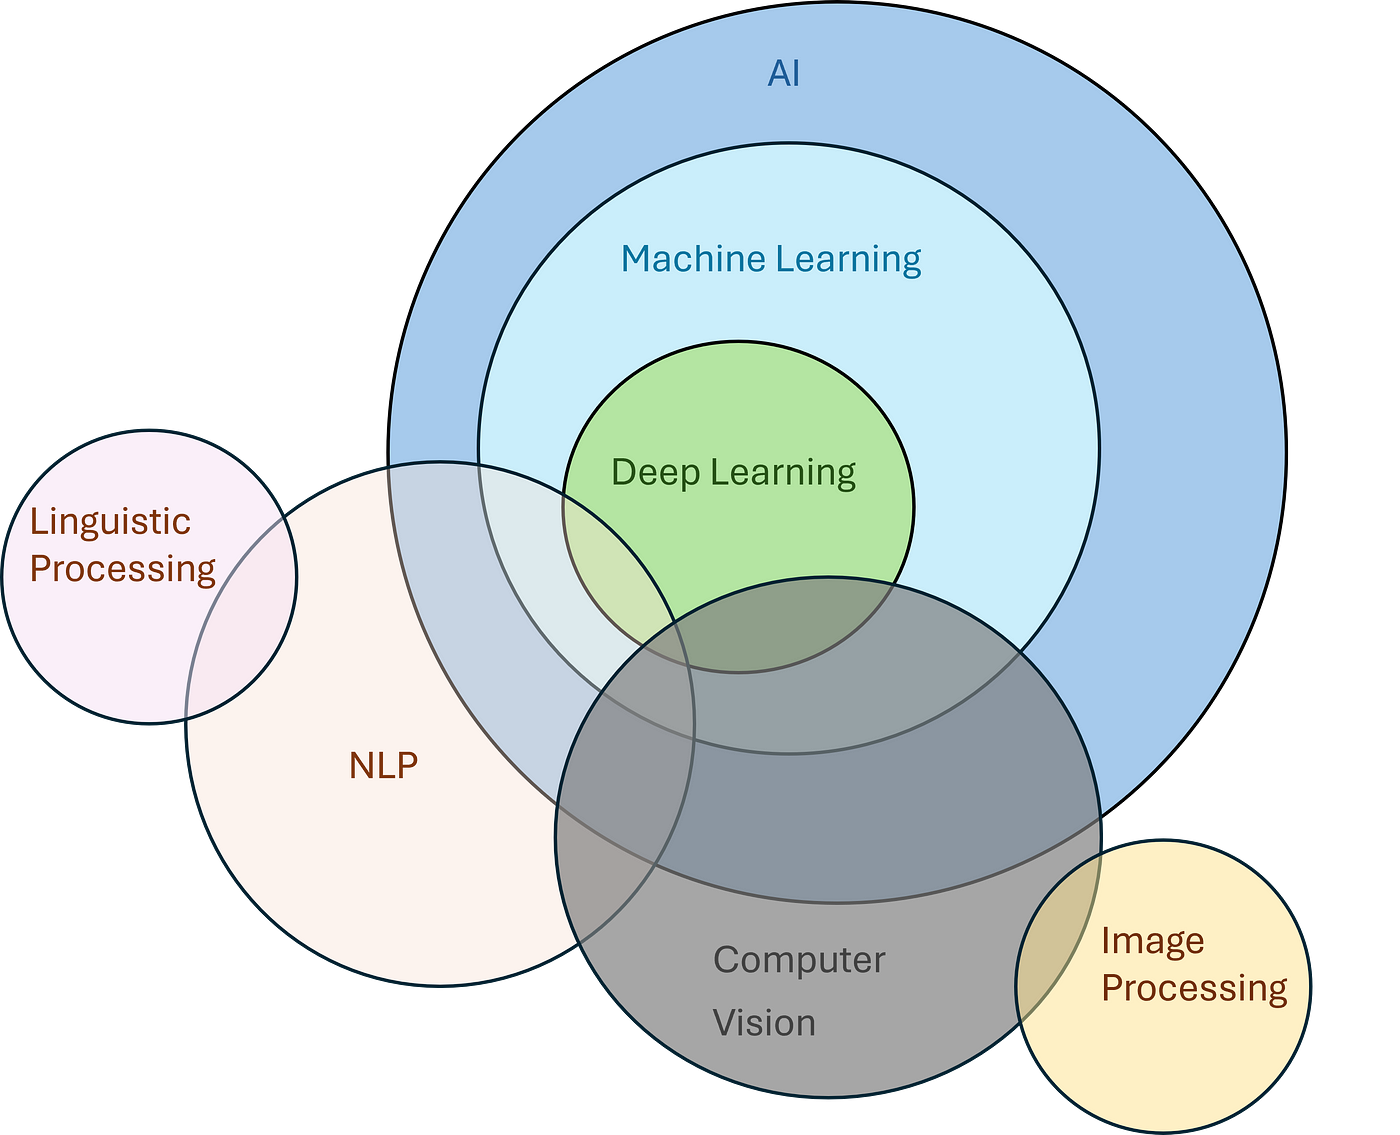
\includegraphics[width=0.8\textwidth]{nlp_venn_diagram.png} 
    \captionof{figure}{Sơ đồ minh họa mối quan hệ giữa NLP và các lĩnh vực liên quan.}
    \label{fig:venn_diagram}
\end{center}

\begin{itemize}
    \item \textbf{Trí tuệ Nhân tạo (Artificial Intelligence - AI):} AI là một ngành khoa học máy tính rộng lớn với mục tiêu tạo ra các cỗ máy thông minh có khả năng suy nghĩ, học hỏi và hành động như con người. Trong bức tranh này, \textbf{NLP là một nhánh con thiết yếu của AI}. Một trí tuệ thực sự toàn diện không thể thiếu khả năng giao tiếp bằng ngôn ngữ tự nhiên. Vì vậy, NLP được xem là một trong những bài toán "AI-hoàn chỉnh" (AI-complete), tức là việc giải quyết hoàn hảo bài toán NLP có thể đồng nghĩa với việc tạo ra một trí tuệ nhân tạo ở cấp độ con người.
    
    \item \textbf{Học máy (Machine Learning - ML):} Học máy là một tập hợp các phương pháp và thuật toán cho phép máy tính "học" từ dữ liệu mà không cần được lập trình một cách tường minh. Trong lịch sử NLP, \textbf{Học máy đã tạo ra một cuộc cách mạng}. Thay vì phải viết tay hàng ngàn quy tắc ngôn ngữ phức tạp và dễ sai sót, các phương pháp học máy cho phép chúng ta xây dựng các mô hình tự động nhận diện các quy luật và mẫu hình (patterns) từ một lượng lớn văn bản. Ngày nay, hầu hết các hệ thống NLP tiên tiến đều được xây dựng trên nền tảng của học máy, và đặc biệt là học sâu (Deep Learning).
    
    \item \textbf{Ngôn ngữ học (Linguistics):} Ngôn ngữ học là ngành khoa học nghiên cứu về chính ngôn ngữ, bao gồm cấu trúc (ngữ pháp), ý nghĩa (ngữ nghĩa), và cách sử dụng trong ngữ cảnh (ngữ dụng). \textbf{Ngôn ngữ học cung cấp nền tảng lý thuyết và kiến thức chuyên môn cho NLP}. Các khái niệm như từ loại (Part-of-Speech), cây cú pháp (syntax tree), cấu trúc hình thái (morphology) đều bắt nguồn từ ngôn ngữ học. Mặc dù các mô hình học sâu hiện đại có thể học được nhiều quy luật ngầm mà không cần kiến thức ngôn ngữ học tường minh, việc hiểu các nguyên lý cơ bản của ngôn ngữ học vẫn cực kỳ quan trọng để thiết kế mô hình, diễn giải kết quả và chẩn đoán lỗi.
\end{itemize}

Nói một cách ví von: AI đặt ra mục tiêu (tạo ra máy móc thông minh), Ngôn ngữ học cung cấp bản đồ và quy luật của "vùng đất" ngôn ngữ, còn Học máy cung cấp những công cụ (xe ủi, máy xúc) để khai phá và xây dựng trên vùng đất đó. NLP chính là công trình được tạo ra từ sự kết hợp của cả ba yếu tố trên.

\subsection{Tổng quan các Kỷ nguyên Phát triển (Luật lệ \(\rightarrow\) Thống kê \(\rightarrow\) Học sâu \(\rightarrow\) Transformer)}
\label{ssec:ky_nguyen_phat_trien}

Lịch sử phát triển của NLP là một câu chuyện hấp dẫn về sự thay đổi trong tư duy và phương pháp luận, được đánh dấu bởi bốn kỷ nguyên chính. Mỗi kỷ nguyên đại diện cho một bước nhảy vọt về khả năng và hiệu suất.

\paragraph{Kỷ nguyên 1: Dựa trên Luật lệ (Symbolic NLP, những năm 1950 -- 1980)}
Đây là giai đoạn sơ khai, chịu ảnh hưởng lớn từ ngôn ngữ học hình thức và logic.
\begin{itemize}
    \item \textbf{Tư duy cốt lõi:} Ngôn ngữ có thể được mô tả hoàn toàn bằng một bộ các quy tắc (rules) và từ điển được tạo ra thủ công bởi các chuyên gia ngôn ngữ.
    \item \textbf{Phương pháp:} Các hệ thống dựa trên ngữ pháp hình thức (formal grammars), phân tích cú pháp bằng tay, và các bộ quy tắc logic phức tạp. Ví dụ kinh điển là hệ thống SHRDLU \cite{winograd1972understanding} có thể đối thoại về một thế giới các khối hộp bằng cách áp dụng các quy tắc logic chặt chẽ.
    \item \textbf{Ưu điểm:} Độ chính xác có thể rất cao trong một lĩnh vực (domain) hẹp và được định nghĩa rõ ràng. Các quy tắc có thể diễn giải được, dễ hiểu tại sao hệ thống đưa ra một kết quả cụ thể.
    \item \textbf{Nhược điểm:} Cực kỳ \textit{giòn} (brittle) -- hệ thống dễ dàng thất bại khi gặp phải một câu nói không tuân theo quy tắc đã định sẵn. Tốn rất nhiều công sức của chuyên gia để xây dựng và bảo trì. Khó mở rộng và thích ứng với các lĩnh vực mới.
\end{itemize}

\paragraph{Kỷ nguyên 2: Dựa trên Thống kê (Statistical NLP, những năm 1990 -- 2010)}
Sự bùng nổ của dữ liệu số và sức mạnh tính toán đã dẫn đến một sự thay đổi mô hình (paradigm shift).
\begin{itemize}
    \item \textbf{Tư duy cốt lõi:} Thay vì cố gắng dạy cho máy tính các quy tắc, hãy để nó tự học các quy luật từ dữ liệu thực tế. Các vấn đề ngôn ngữ được định hình lại thành các bài toán dự đoán dựa trên xác suất. Câu nói nổi tiếng của Frederick Jelinek đã tóm gọn tinh thần của thời kỳ này: "Mỗi lần tôi sa thải một nhà ngôn ngữ học, hiệu suất của hệ thống nhận dạng giọng nói lại tăng lên."
    \item \textbf{Phương pháp:} Mô hình N-gram, Mô hình Markov ẩn (HMM) \cite{rabiner1989tutorial}, Hồi quy Logistic, Máy Vector Hỗ trợ (SVM) \cite{cortes1995support}, và sau này là Các trường Ngẫu nhiên Có điều kiện (CRF) \cite{lafferty2001conditional}. Các khái niệm như TF-IDF trở thành tiêu chuẩn để biểu diễn văn bản.
    \item \textbf{Ưu điểm:} Mạnh mẽ (robust) và linh hoạt hơn nhiều so với hệ thống luật. Có khả năng xử lý ngôn ngữ tự nhiên "trong đời thực" với tất cả sự lộn xộn của nó.
    \item \textbf{Nhược điểm:} Gặp vấn đề với \textit{sự thưa thớt của dữ liệu} (data sparsity), đặc biệt là với các N-gram dài. Khó nắm bắt được ý nghĩa ngữ nghĩa sâu sắc và các mối quan hệ phụ thuộc tầm xa trong câu.
\end{itemize}

\paragraph{Kỷ nguyên 3: Dựa trên Học sâu (Deep Learning, khoảng 2013 -- 2017)}
Cuộc cách mạng thực sự bắt đầu khi các mạng nơ-ron sâu được áp dụng vào NLP.
\begin{itemize}
    \item \textbf{Tư duy cốt lõi:} Tự động học các biểu diễn (representations) hoặc các đặc trưng (features) của từ và câu dưới dạng các vector dày đặc (dense vectors), hay còn gọi là \textit{embeddings}. Các biểu diễn này nắm bắt được các mối quan hệ ngữ nghĩa và cú pháp một cách hiệu quả.
    \item \textbf{Phương pháp:} Word2Vec \cite{mikolov2013efficient}, GloVe \cite{pennington2014glove} tiên phong trong việc học biểu diễn từ. Các kiến trúc như Mạng Nơ-ron Hồi tiếp (RNN), LSTM \cite{hochreiter1997long}, GRU \cite{cho2014learning} trở nên thống trị trong các bài toán xử lý chuỗi. Mô hình Chuỗi-sang-Chuỗi (Seq2Seq) \cite{sutskever2014sequence} kết hợp với cơ chế Chú ý (Attention) \cite{bahdanau2014neural} đã tạo ra bước đột phá trong dịch máy.
    \item \textbf{Ưu điểm:} Đạt hiệu suất vượt trội trên hầu hết các benchmark. Có khả năng nắm bắt ngữ cảnh và ngữ nghĩa tốt hơn nhiều so với các mô hình thống kê.
    \item \textbf{Nhược điểm:} RNN vẫn gặp khó khăn trong việc xử lý các phụ thuộc tầm rất xa. Việc huấn luyện tuần tự của RNN làm hạn chế khả năng song song hóa, gây tốn thời gian.
\end{itemize}

\paragraph{Kỷ nguyên 4: Kỷ nguyên Transformer (The Transformer Era, 2017 -- Hiện tại)}
Bài báo "Attention Is All You Need" \cite{vaswani2017attention} vào năm 2017 đã khai sinh ra một kiến trúc mới và định hình lại toàn bộ lĩnh vực.
\begin{itemize}
    \item \textbf{Tư duy cốt lõi:} Hoàn toàn từ bỏ kiến trúc hồi tiếp (recurrence) và tích chập (convolution), thay vào đó chỉ dựa vào cơ chế \textit{tự chú ý (self-attention)} để nắm bắt mối quan hệ giữa các từ trong một chuỗi.
    \item \textbf{Phương pháp:} Kiến trúc Transformer gốc, và sau đó là sự bùng nổ của các Mô hình Ngôn ngữ Lớn (Large Language Models - LLMs) được huấn luyện trước (pre-trained) trên một lượng dữ liệu khổng lồ, ví dụ như BERT \cite{devlin2018bert}, GPT \cite{radford2018improving,radford2019language,brown2020language}, T5 \cite{raffel2020exploring}, Llama \cite{touvron2023llama}.
    \item \textbf{Ưu điểm:} Khả năng song song hóa cao, cho phép huấn luyện các mô hình cực lớn. Hiệu quả vượt trội trong việc xử lý các phụ thuộc tầm xa. Mô hình "nền tảng" (foundation model) được huấn luyện trước có thể được tinh chỉnh (fine-tune) cho nhiều tác vụ khác nhau với hiệu quả đáng kinh ngạc, dẫn đến sự phát triển của học ít mẫu (few-shot learning) và học không cần mẫu (zero-shot learning).
    \item \textbf{Nhược điểm:} Đòi hỏi tài nguyên tính toán và dữ liệu cực lớn. Các vấn đề về diễn giải, thiên kiến, và đạo đức trở nên nổi cộm hơn bao giờ hết.
\end{itemize}